\documentclass[border=10pt]{standalone}
\usepackage{pgfplots}
\pgfplotsset{compat=1.18}
\usepgfplotslibrary{groupplots,fillbetween}
\begin{document}
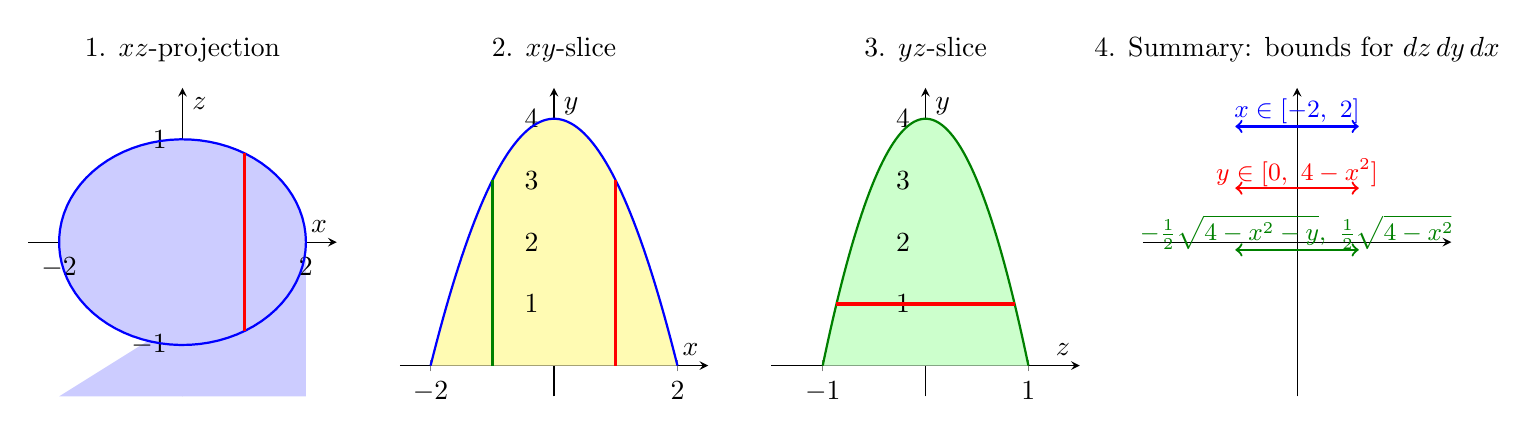
\begin{tikzpicture}
\begin{groupplot}[
    group style={group size=4 by 1, horizontal sep=0.8cm},
    width=5.5cm, height=5.5cm,
    axis lines=middle,
]

% Step 1: xz-projection (ellipse)
\nextgroupplot[
    xlabel={$x$}, ylabel={$z$},
    title={1. $xz$-projection},
    xmin=-2.5, xmax=2.5, ymin=-1.5, ymax=1.5,
]
\addplot[name path=A, blue, thick, domain=0:2*pi, samples=80] ({2*cos(deg(x))}, {sin(deg(x))});
\addplot[name path=B, draw=none, domain=-2:2, samples=2] {-1.5};
\addplot[blue!20] fill between[of=A and B];
\addplot[red, very thick, domain=-0.866:0.866, samples=10] ({1}, {x});

% Step 2: xy-slice
\nextgroupplot[
    xlabel={$x$}, ylabel={$y$},
    title={2. $xy$-slice},
    xmin=-2.5, xmax=2.5, ymin=-0.5, ymax=4.5,
    ytick={1,2,3,4},
]
\addplot[name path=A, blue, thick, domain=-2:2, samples=80] {4 - x^2};
\addplot[name path=B, draw=none, domain=-2:2, samples=2] {0};
\addplot[yellow!30] fill between[of=A and B];
\addplot[red, very thick, domain=0:3, samples=10] ({1}, {x});
\addplot[green!50!black, very thick, domain=0:3, samples=10] ({-1}, {x});

% Step 3: yz-slice
\nextgroupplot[
    xlabel={$z$}, ylabel={$y$},
    title={3. $yz$-slice},
    xmin=-1.5, xmax=1.5, ymin=-0.5, ymax=4.5,
    ytick={1,2,3,4},
]
\addplot[name path=A, green!50!black, thick, domain=-1:1, samples=80] {4 - 4*x^2};
\addplot[name path=B, draw=none, domain=-1:1, samples=2] {0};
\addplot[green!20] fill between[of=A and B];
\addplot[red, very thick, domain=-0.866:0.866, samples=10] ({x}, {1});

% Step 4: Bounds summary (separate text)
\nextgroupplot[
    title={4. Summary: bounds for $dz\,dy\,dx$},
    xmin=-1, xmax=1, ymin=-1, ymax=1,
    enlargelimits=false,
    xtick=\empty, ytick=\empty,
]
\node[blue, anchor=center] at (axis cs:0, 0.85) {\small $x \in [-2,\ 2]$};
\draw[blue, thick, <->] (-0.4, 0.75) -- (0.4, 0.75);
\node[red, anchor=center] at (axis cs:0, 0.45) {\small $y \in [0,\ 4-x^2]$};
\draw[red, thick, <->] (-0.4, 0.35) -- (0.4, 0.35);
\node[green!50!black, anchor=center] at (axis cs:0, 0.05) {\small $z \in \left[-\frac{1}{2}\sqrt{4-x^2-y},\ \frac{1}{2}\sqrt{4-x^2-y}\right]$};
\draw[green!50!black, thick, <->] (-0.4, -0.05) -- (0.4, -0.05);

\end{groupplot}
\end{tikzpicture}
\end{document}